\chapter{Elektromagnetische Felder in Substanzen}

Bisher haben wir die mikroskopischen \textsc{Maxwell}-Gleichungen betrachtet, die im Vakuum auch auf makroskopischen Längenskalen ihre Gültigkeit behalten. Dabei haben wir angenommen, dass $\rho$ und $\vec{j}$ alle Quellen enthalten. \\
Um nun den Schritt zu Betrachtung von Feldern in Substanzen zu machen, müssen wir weitere Feldquellen (Polarisationsladungen, Abschirmströme) betrachten.

\section{Elektrische Polarisation}

Man stellt fest, dass sich die makroskopische Ladungsdichte 
\begin{equation*}
\rho = \rho_0 + \rho_p
\end{equation*}
aus der Dichte der freien Ladungen $\rho_0$ und der der sogenannten \textbf{Polarisationsladungen} $\rho_P$ zusammensetzt. Letztere werden durch ein äußeres Feld induziert und sind im Experiment allgemein nicht bekannt. \\
Aufgrund der Ladungserhaltung muss die Polarisationsladung im \emph{gesamten }Raum verschwinden.
\begin{equation*}
\rho_P\neq 0, \qquad \text{aber}\quad \int\mathrm{d}V \rho_P = Q_P = 0
\end{equation*}
Das ist insofern intuitiv, da ein äußeres Feld Ladungen voneinander trennen und somit lokal Dichteschwankungen hervorrufen, aber nie Ladungen vernichten kann. \\
Auch die Polarisationsladungen erfüllen die Kontinuitätsgleichung, die so zur Definition der \textbf{Polarisationsstromdichte} $\vec{j}_P$ dient.
\begin{equation*}
\dot{\rho}_P+\div\vec{j}_P=0
\end{equation*}
Wir erhalten so 
\begin{equation*}
\rho_P = -\nabla\underbrace{\int\limits_0^t\mathrm{d}t'\ \vec{j}_P}_{\vec{=:P}} + \underbrace{\rho_P(0)}_{=0}.
\end{equation*}
Wobei wir $\vec{P}$ als \textbf{elektrische Polarisation} bezeichnen wollen.
\begin{empheq}[box=\highlightbox]{align*}
\vec{P} &=\int\vec{j}_P\mathrm{d}t\\
\rho_P &= -\div\vec{P}\\
Q_P &=-\int\mathrm{d}V\ \nabla\vec{P}=-\oiint\mathrm{d}\vec{A}_F\cdot\vec{P}=0
\end{empheq}
Nun gilt aber außerdem
\begin{equation*}
\int\vec{j}_P\mathrm{d}V = \int\d V\dot{\vec{P}} = \dot{\vec{p}}.
\end{equation*}
Man sieht, dass man die Polarisation auch als \textbf{Dipoldichte} auffassen kann. Das wollen wir anhand des Potentials einer Polarisationsladungsverteilung nachprüfen.
\begin{align*}
\varphi_P(\vec{r}) &=\frac{1}{4\pi\epsilon_0} \int\mathrm{d}V'\ \frac{\rho_P(\vec{r'})}{|\vec{r}-\vec{r}'|} = -\frac{1}{4\pi\epsilon_0}\int\mathrm{d}V'\ \frac{1}{|\vec{r}-\vec{r}'|}\nabla_{\vec{r}'}\vec{P}(\vec{r}') = \\
&=\frac{1}{4\pi\epsilon_0}\int\mathrm{d}V'\ \vec{P}(\vec{r}')\cdot\nabla_{\vec{r}'}\frac{1}{|\vec{r}-\vec{r}'|} =-\frac{1}{4\pi\epsilon_0}\int\mathrm{d}V' \vec{P}(\vec{r}')\nabla_{\vec{r}'}\frac{1}{|\vec{r}-\vec{r}'|}
\end{align*}
Vergleicht man das mit dem Potential eines Dipols
\begin{equation*}
\varphi(\vec{r})=-\frac{1}{4\pi\epsilon_0}\cdot\vec{p}\cdot\nabla\frac{1}{r},
\end{equation*}
so bestätigt sich unsere Auffassung. Makroskopisch entspricht die elektrische Polarisation also:
\begin{empheq}[box=\highlightbox]{equation*}
\vec{P} = \diff{\vec{p}}{V} \vphantom{\Big|}
\end{empheq}
Auf atomarer Ebene sind die Dipolmomente natürlich nicht kontinuierlich, sondern diskret verteilt. In diesem Fall muss zur Summe übergegangen werden.
\begin{equation*}
\vec{P} = \frac{1}{|V|}\sum\limits_{i\in V}\vec{p}_i
\end{equation*}
Da wir nun die Polarisationsladungen durch die Dipoldichte ausdrücken können, wird die erste \textsc{Maxwell}-Gleichung zu
\begin{equation*}
\epsilon_0\div\vec{E}=\rho_0+\rho_p = \rho_0 - \div\vec{P}.
\end{equation*}
Nach umstellen erhalten wir die erste makroskopische \textsc{Maxwell}-Gleichung
\begin{align*}
\div\left(\epsilon_0\vec{E}+\vec{P}\right)&=\rho_0\\
\div\vec{D} &= \rho_0 ,
\end{align*}
wobei $\vec{D} = \epsilon_0\vec{E} +\vec{P}$ das \textbf{elektrische Verschiebefeld} ist, das allein von den freien Ladungen $\rho_0$ abhängt.

\section{Magnetisierung}

Im makroskopischen Fall setzt sich auch die Stromdichte aus mehreren Quellen zusammen.
\begin{equation*}
\vec{j} = \underbrace{\vec{j}_k+\vec{j}_l}_{\vec{j}_0} + \vec{j}_P + \vec{j}_M
\end{equation*}
Dabei ist $\vec{j}_k$ der Konvektionsstrom bewegter Teilchen, $\vec{j}_l$ der Leitungsstrom, $\vec{j}_P$ der Polarisationsstrom und $\vec{j}_M$ ein Strom ohne Ladungstrennung. \\
Die Kontinuitätsgleichung lautet
\begin{equation*}
\dot{\rho}+\div\vec{j} = \dot{\rho}_0 + \dot{\rho}_P + \div\vec{j}_0 + \div\vec{j}_P + \div\vec{j}_M = 0.
\end{equation*}
Da $\vec{j}_0$ und $\vec{j}_P$ jeweils separat eine Kontinuitätsgleichung erfüllen, muss $\div\vec{j}_M=0$ sein. Ein Magnetisierungsstrom hat also keine Ladungsträger. Da er divergenzfrei ist, können wir mit Einführung der Magnetisierung $\vec{M}$
\begin{empheq}[box=\highlightbox]{equation*}
\vec{j}_M  = \rot\vec{M}\vphantom{\big|}
\end{empheq}
schreiben.\\
Das resultierende Vektorpotential ist dann
\begin{align*}
\vec{A}_M(\vec{r}) &= \frac{\mu_0}{4\pi}\int\mathrm{d}V'\  \frac{\vec{j}_M(\vec{r}')}{|\vec{r}-\vec{r}'|} = \frac{\mu_0}{4\pi}\int\frac{\mathrm{d}V'}{|\vec{r}-\vec{r}'|}\nabla_{\vec{r}'}\times\vec{M}(\vec{r}') = \\
&=-\frac{\mu_0}{4\pi}\int\mathrm{d}V'\ \vec{M}(\vec{a}')\times\nabla_{\vec{r}'}\frac{1}{|\vec{r}-\vec{r}'|}
\end{align*}
Vergleichen wir das nun wieder mit dem magnetischen Dipolpotential
\begin{equation*}
\vec{A}(\vec{r}) = -\frac{\mu_0}{4\pi}\vec{m}\times\nabla\frac{1}{r},
\end{equation*}
so können wir analog zum elektrischen Fall, die Magnetisierung als \textbf{magnetische Dipoldichte} auffassen:
\begin{empheq}[box=\highlightbox]{equation*}
\vec{M} = \diff{\vec{m}\vphantom{\big|}}{V\vphantom{\big|}}
\end{empheq}
Daraus ergibt sich nun mit
\begin{equation*}
\frac{1}{\mu_0}\rot\vec{B}=\vec{j} + \epsilon_0\dot{\vec{E}} = \vec{j}_0 + \dot{\vec{P}} + \rot\vec{M} + \epsilon_0\dot{\vec{E}}
\end{equation*}
das \textbf{\textsc{Ampére}sche Gesetz für Substanzen}
\begin{align*}
\rot\left(\frac{\vec{B}}{\mu_0}-\vec{M}\right) & = \vec{j}_0 + \pdiff{}{t}\left(\epsilon_0\vec{E}+\vec{P}\right)\\
\rot\vec{H} &= \vec{j}_0 + \dot{\vec{D}}.
\end{align*}
Zusammengefasst erhalten wir so die makroskopischen \textsc{Maxwell}-Gleichungen
\begin{empheq}[box=\highlightbox]{align*}
\vphantom{\big|}\div\vec{B} &=0 &\div\vec{D} &= \rho_0\\
\rot \vec{E} + \dot{\vec{B}} &= 0 &\rot \vec{H}-\dot{\vec{D}}&=\vec{j}_0
\end{empheq}
mit den Materialeigenschaften
\begin{empheq}[box=\highlightbox]{align*}
\vec{D}&=\epsilon_0\vec{E}+\vec{P} &\vec{H} &= \frac{\vec{B}\vphantom{\big|}}{\mu_0\vphantom{\big|}} -\vec{M}.
\end{empheq}

\section{Materialgesetze}

Sowohl Polarisation $\vec{P}$, Magnetisierung $\vec{M}$ als auch der Leitungsstrom $\vec{j}_l$ werden durch die Felder $\vec{E}$ und $\vec{B}$ hervorgerufen und sind im allgemeinen materialabhängig, insbesondere auch von Druck und Temperatur. Häufig erhält man jedoch einfache Gesetze, die abgebrochenen \textsc{Taylor}-Entwicklungen entsprechen, also für Felder gültig sind, die schwach gegen die interatomaren Kräfte sind.\\
Dazu wollen wir ein paar einfache Beispiele betrachten.

\begin{enumerate}
	\item \textbf{\textsc{Ohm}'sches Gesetz}
	\begin{equation*}
	I = \vec{A}_F\cdot\vec{j} = A_F\sigma E = A_F\sigma\frac{U}{l} = \frac{U}{R}
	\end{equation*}
	\item \textbf{Verschiebefeld}
	\begin{equation*}
	\vec{D}=\epsilon_0\vec{E}+\vec{P}=(1+\chi_l)\epsilon_0\vec{E}=\epsilon_0\epsilon_r \vec{E}
	\end{equation*}
	\item \textbf{Magnetische Dipoldichte}
	\begin{equation*}
	\vec{H} = \frac{1}{\mu_0}\vec{B}-\vec{M} = (1-\chi_m)\frac{1}{\mu_0}\vec{B}  = \frac{1}{\mu_0\mu_r}\vec{B}
	\end{equation*} 
\end{enumerate}

So werden die \textsc{Maxwell}-Gleichungen mit linearen Materialgesetzen zu
\begin{align*}
\div\vec{B}&=0 &\div(\epsilon_0\epsilon_r\vec{E})&=\rho_0\\
\rot \vec{E}+\dot{\vec{B}}&=0 &\rot\frac{\vec{B}}{\mu_0}-\epsilon_0\epsilon_r\dot{\vec{E}}&=\vec{j}_0.
\end{align*}

Natürlich können $\mu=\mu_0\mu_r$ und $\epsilon=\epsilon_0\epsilon_r$ auch richtungsabhängig sein und müssen dann durch Tensoren $\tens{\mu}$ und $\tens{\epsilon}$ ausgedrückt werden.\\

Untersuchen wir nun, wie sich uns bereits aus dem Vakuum bekannte Größen in Substanzen verhalten.
\begin{enumerate}
		\item \textbf{Phasengeschwindigkeit}
		\begin{equation*}
		u_P=\frac{\omega}{k}=\frac{1}{\sqrt{\mu\epsilon}}=\frac{c}{\sqrt{\mu_r\epsilon_r}} =: \frac{c}{n}\quad\quad\text{mit}\ n=\sqrt{\mu_r\epsilon_r}
		\end{equation*}
		\item \textbf{Energiedichte}
		\begin{equation*}
		w=\frac{\epsilon}{2}E^2 + \frac{1}{2\mu}B^2 = \frac{1}{2}\left(\vec{D}\cdot\vec{E}+\vec{B}\cdot\vec{H}\right)
		\end{equation*}
		\item \textbf{Energiestromdichte}
		\begin{equation*}
		\vec{S}_P = \frac{1}{\mu}\vec{E}\times\vec{B} = \vec{E}\times\vec{H}
		\end{equation*}
		\item \textbf{Impulsdichte}
		\begin{equation*}
		\vec{g}=\epsilon\vec{E}\times\vec{B}=\vec{D}\times\vec{B}=\frac{u_P^2}{c^2}\vec{S}_P
		\end{equation*}
\end{enumerate}
Es ist zu beachten, dass die Ausdrücke, die auf die Hilfsfelder zurückgreifen nur für lineare Medien Richtigkeit haben.
\newpage
\section{Verhalten an Grenzflächen}

\begin{wrapfigure}[]{r}[0cm]{0cm}
	\raisebox{0pt}[\dimexpr\height-1\baselineskip\relax]{
		\colorbox{hgrey}{
			\begin{tikzpicture}
			\draw(0,0)-- (0,4) ;
			\draw[|-|] (2,0.5)--node[right]{$A_F / L$}(2,3.5);
			\draw[ultra thick] (-1,0.5)--(1,0.5);
			\draw[ultra thick] (-1,3.5)--(1,3.5);
			\draw[ultra thick] (-1,0.5)--(-1,3.5);
			\draw[ultra thick] (1,0.5)--(1,3.5);
			\draw[|-|] (-1,-0.5)--node[below]{$d\rightarrow 0$}(1,-0.5);
			\draw (-1.5,4.5) node{\textbf{1}};
			\draw (1.5,4.5) node{\textbf{2}};
			\draw[color=hgrey] (-2.3,4.5) node{f};
			\draw[->] (0,2)--(0.5,2) node[below]{$\vec{n}$};
			\draw[->] (-2,2)--(-2,2.5) node[left]{$\vec{t}$};
			\fill[pattern=north east lines] (0,0)--(0,4)--(-0.5,4)--(-0.5,0);
			\end{tikzpicture}
		}
	}
	\caption{Integrationsvolumen  bzw. Fläche}
\end{wrapfigure}
Wir wollen nun das Verhalten der Felder an Grenzflächen zwischen zwei Medien untersuchen. Dazu definieren wir uns ein unendlich flaches Integrationsvolumen, das den Übergang zwischen den beiden Substanzen einschließt.\\
Aus der Quellenfreiheit des $B$-Feldes folgt
\begin{equation*}
\oiint\mathrm{d}\vec{A}_F\cdot\vec{B}=0
\end{equation*}
Wir halten die Fläche $A_F$ konstant und da die Quellenfreiheit für alle Volumina gilt, muss 
\begin{equation*}
\vec{n}A_F(\vec{B}_2-\vec{B}_1) = A_F(B_{2n}-B_{1n}) = 0
\end{equation*}
sein. Daraus können wir ablesen, dass die Normalkomponente von $\vec{B}$ beim Grenzübergang zwischen zwei Medien stetig sein muss.\\

Die elektrische Polarisation $\vec{D}$ enthält als Quellen die freien Ladungen $Q_0$. Analog zu oben erhalten wir durch dieselben Überlegungen jedoch
\begin{equation*}
D_{2n}-D_{1n}=\frac{Q_0}{A_F}=\sigma_0.
\end{equation*}

$\vec{D}$ ist also nur stetig an Grenzflächen, wenn es keine Oberflächenladungen gibt.\\

Ähnlich zum obigen Integrationsvolumen verwenden wir nun eine Fläche mit fast verschwindender Breite $d\rightarrow 0$, und der Höhe $L$, die parallel zu $\vec{n}$ aus der Fläche zeigt - man stelle sich Abbildung 9.1 mit $L$ statt $A_F$ vor.\\

Wir nehmen an, dass sich das Magnetfeld über die Zeit nicht ändert ($\dot{\vec{B}}=0$), so erhalten wir aus $\rot \vec{E} = 0$
\begin{equation*}
\oint\mathrm{d}\vec{r}\cdot\vec{E} = 0 
\end{equation*}
und damit
\begin{equation*}
\vec{t}L(\vec{E}_2-\vec{E}_1)=L(E_{2t}-E_{1t})=0.
\end{equation*}
Die Tangentialkomponente von $\vec{E}$ ist also genau dann stetig, wenn $\vec{B}$ zeitunabhängig ist. \\

Nun gehen wir davon aus, dass sich die Dipoldichte zeitlich nicht ändert ($\dot{\vec{D}}=0$) und erhalten so analog aus $\rot \vec{H}=\vec{j}_0$
\begin{equation*}
L(H_{2t}-H_{1t})=I_{0,\parallel},
\end{equation*}
wobei $I_{0,\parallel}$ der Anteil des Stroms entlang der Grenzfläche ist. $\vec{H}$ ist also stetig, wenn an der Oberfläche keine Ströme fließen und $\vec{D}$ zeitunabhängig ist.\\
Für $\vec{B}$ ergibt sich unter Berücksichtigung der Magnetisierungsströme
\begin{equation*}
\frac{L}{\mu_0}(B_{2t}-B_{1t})=I_{0,\parallel}+I_{M,\parallel}.
\end{equation*}
Für stromfreie Grenzflächen gilt also
\begin{equation*}
\Delta B_{t} = \mu_0\frac{I_{M,\parallel}}{L}.
\end{equation*}

Dieselben Ergebnisse für $E_t$ hätte man auch aus der Überlegung heraus erzielt, dass im Falle statischer Felder ($\dot{\vec{D}}=0,\ \dot{\vec{B}}=0$) das Potential stetig sein muss. Es muss nämlich gelten
\begin{align*}
\left.\varphi_1(\vec{r})\right|_\text{Grenzfl.} &= \left.\varphi_2(\vec{r})\right|_\text{Grenzfl.}\\
\varphi_1(\vec{r}+\mathrm{d}\vec{r}) &=\varphi_2(\vec{r}+\mathrm{d}\vec{r})	\\
\Rightarrow
\pdiff{\varphi_1}{\vec{t}} &=\pdiff{\varphi_2}{\vec{t}}\\
E_{1t} &= E_{2t}
\end{align*}

i) \textbf{ Plattenkondensator mit Dielektrikum}\\

\begin{wrapfigure}[]{l}[0cm]{0cm}
	\raisebox{0pt}[\dimexpr\height-1\baselineskip\relax]{
		\colorbox{hgrey}{
			\begin{tikzpicture}
			%Platten
			\draw[ultra thick] (0,0)--(0,3);
			\draw[ultra thick] (3,0)--(3,3);
			\draw (0,1.5)--(3,1.5);
			\fill[opacity=0.2,pattern=north east lines] (0,0)--(3,0)--(3,1.5)--(0,1.5);

			%Felder
			\draw[->](0,2)--node[above]{$\vec{E}_1$}(2.9,2);
			\draw[->](0,0.5)--node[above]{$\vec{E}_2$}(2.9,0.5);
			
			%Ladungen
			\draw (-0.5,0.5) node{+};
			\draw (-0.5,2) node{+};
			\draw (3.5,0.5) node{-};
			\draw (3.5,2) node{-};
			\end{tikzpicture}
		}
	}
	\caption{Kondensator unten gefüllt}
\end{wrapfigure}

Die Tangentialkomponente von $\vec{E}$ muss stetig sein, da sich $\vec{B}$ nicht ändert. Die Polarisation muss jedoch für $\epsilon_1\neq\epsilon_2$ in beiden Bereichen unterschiedlich groß sein.\\ \linebreak\linebreak\linebreak\linebreak\linebreak\linebreak\linebreak

\begin{wrapfigure}[]{r}[0cm]{0cm}
	\raisebox{-.5cm}[\dimexpr\height-1\baselineskip\relax]{
		\colorbox{hgrey}{
			\begin{tikzpicture}
			%Platten
			\draw[ultra thick] (0,0)--(0,3);
			\draw[ultra thick] (3,0)--(3,3);
			\draw (1.5,0)--(1.5,3);
			\fill[opacity=0.2,pattern=north east lines] (1.5,0)--(3,0)--(3,3)--(1.5,3);
			
			%Felder
			\draw[->](0,2)--node[above]{$\vec{E}_1$}(1.4,2);
			\draw[->](0,.5)--(1.4,.5);
			\draw[->](1.5,2)--node[above]{$\vec{E}_2$}(2.9,2);
			\draw[->](1.5,.5)--(2.9,.5);
			
			%Ladungen
			\draw (-0.5,0.5) node{+};
			\draw (-0.5,2) node{+};
			\draw (3.5,0.5) node{-};
			\draw (3.5,2) node{-};
			\end{tikzpicture}
		}
	}
	\caption{Kondensator rechts gefüllt}
\end{wrapfigure}
Da $D_n$ aufgrund der fehlenden Oberflächenladungen stetig  ist, müssen die E-Felder unterschiedlich groß sein.\\ \linebreak\linebreak\linebreak\linebreak\linebreak

ii) \textbf{ Grenzfläche schräg zu den Feldlinien}\\

\begin{wrapfigure}[10]{l}[0cm]{0cm}
	\raisebox{0pt}[\dimexpr\height-1\baselineskip\relax]{
		\colorbox{hgrey}{
			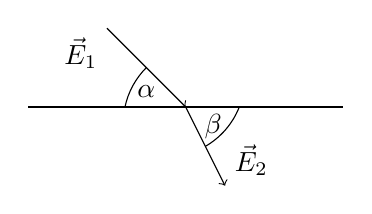
\begin{tikzpicture}
			\draw (-2,0)--(2,0);
			\draw[->] (-1,1)node[below left]{$\vec{E}_1$}--(0,0);
			\draw (-0.5,0.5) arc(135:168:1cm);
			\draw (-0.5,0.4) node[below]{$\alpha$};
			\draw[->] (0,0)--(0.5,-1)node[above right]{$\vec{E}_2$};
			\draw (0.25,-0.5) arc(-60:-22:1cm);
			\draw (0.35,-0.25) node{$\beta$};
			\end{tikzpicture}
		}
	}
	\caption{schräge Feldlinien}
\end{wrapfigure}
Aus der Stetigkeit der Tangetialkomponente von $\vec{E}$ und der Normalkomponente von $\vec{D}$ folgt
\begin{align*}
E_{1t}&=E_{2t} &\Rightarrow& & E_1\sin\alpha &=E_2\sin\beta\\
D_{1n}&=D_{2n} &\Rightarrow& &\epsilon_1E_1\cos\alpha &= \epsilon_2E_2\cos\beta.
\end{align*}
Diese beiden Gleichungen können wir dividieren und erhalten
\begin{equation*}
\frac{\tan\alpha}{\tan\beta}=\frac{\epsilon_1}{\epsilon_2}.
\end{equation*}\\


\underline{\textbf{Beispiel}}
\ \\
\ \\
\textbf{Dielektrische Kugel im homogenen Feld}\\
\ \\

Eine dielektrische Kugel mit Radius $a$ möge sich in einem homogenen elektrischen Feld $\vec{E}_0$ befinden. Wir legen den Koordinatenursprung in die Kugelmitte. 
\begin{align*}
\rot \vec{E} &=0 &\Rightarrow & &\vec{E}=-\grad\varphi\\
\div\vec{D} &=0 &\Rightarrow& &-\div(\epsilon \ \grad\varphi)=0
\end{align*}
Wenn das Potential an der Grenzfläche $r=a$ stetig ist, dann ist es auch $E_t$. Ebenso ist $\epsilon\pdiff{\varphi}{r}$ stetig, wenn $D_n$ stetig ist. Wir wählen deshalb ähnlich wie in Kapitel 3.7 den Ansatz
\begin{equation*}
\varphi(\vec{r})=-\vec{E}_0\cdot\vec{r}\cdot g(r,a,\epsilon_i,\epsilon_a).
\end{equation*}
Durch Separation erhalten wir
\begin{equation*}
\frac{4}{r}\diff{g}{r}+\ddiff{g}{r}=0
\end{equation*}
und schließlich
\begin{equation*}
g(r)=\begin{cases}
\alpha + \beta\frac{a^3}{r^3} \qquad&\text{für}\ r<a\\
\gamma + \delta\frac{a^3}{r^3}\qquad&\text{für}\ r>a
\end{cases}
\end{equation*}
Aus den Randbedingungen, dass $g(r=0)$ regulär, $g(r\rightarrow a)=1$ und $\varphi$ stetig sein, muss folgt jeweils $\beta=1$, $\gamma=1$ und $\alpha=1+\delta$. Da
\begin{equation*}
\left.\pdiff{\varphi}{r}\right|_\text{Kugeloberfl.} = -\pdiff{}{r}\left(\vec{E}_0\cdot\vec{n}\cdot r\cdot g(r)\right)
\end{equation*}
muss $D_n$ stetig sein. Das heißt also
\begin{equation*}
\epsilon_i \alpha = \epsilon_i(1+\delta)\ \stackrel{!}{=}\ \epsilon_a(1-2\delta).
\end{equation*}
Das können wir eindeutig nach $\alpha$ und $\delta$ auflösen und erhalten
\begin{align*}
\delta & = \frac{\epsilon_a-\epsilon_i}{\epsilon_i+2\epsilon_a}, &\alpha &=\frac{3\epsilon_a}{\epsilon_i+2\epsilon_a}.
\end{align*}
womit wir das Potential bestimmt hätten.
\begin{equation*}
\varphi(r)=\begin{cases}
-\vec{E}_0\cdot\vec{r}\ (1+\delta) \qquad\ &\text{für}\ r<a\\
-\vec{E}_0\cdot\vec{r}  (1+\delta\frac{a^3}{r^3})\quad &\text{für}\ r>a
\end{cases}
\end{equation*}
Das Feld im inneren der Kugel ist
\begin{equation*}
\vec{E}_i = \vec{E}_0(1+\delta) = \vec{E}_0 + \Delta\vec{E}_i,
\end{equation*}
wobei
\begin{equation*}
\Delta\vec{E}_i = \frac{\epsilon_a-\epsilon_i}{\epsilon_i+2\epsilon_a}\vec{E}_0
\end{equation*}
ein entelektrisierendes Feld ist. Analog gilt
\begin{equation*}
\vec{D}_i = \epsilon_i\vec{E}_i = 3\frac{\epsilon_i}{\epsilon_i+2\epsilon_a}\vec{D}_0.
\end{equation*}
Der Außenraum der Kugel sieht natürlich bis auf das homogene äußere Feld aus, wie das Feld eines Dipols mit dem Moment
\begin{equation*}
\vec{p} = -4\pi\epsilon_0\vec{E}_0\delta a^3
\end{equation*}
Es gibt einige Spezialfälle zu betrachten. Im Fall, dass $\epsilon_i$ unendlich groß wird, verschwindet das Feld im Inneren der Kugel. Es wird $\delta=-1$ und das Potential im Außenraum zu
\begin{equation*}
\varphi_a(r)=\vec{E}_0\cdot\vec{r}\left(1-\frac{a^3}{r^3}\right).
\end{equation*}
Das sieht genauso aus, wie das Potential einer leitenden Kugel. Ein Leiter ist also nicht anderes als ein Dielektrikum mit $\epsilon\rightarrow\infty$.\\
Sollte $\epsilon_a=\epsilon_0$ sein (wie im Vakuum), so wird das Entelektrisierungsfeld
\begin{equation*}
\Delta\vec{E}_i=-\frac{\epsilon_i-\epsilon_0}{\epsilon_i+2\epsilon_0}\vec{E}_0
\end{equation*}
und die Polarisation
\begin{align*}
\vec{P}_i &= \vec{D}_i - \epsilon_0\vec{E}_i = -3\epsilon_0\Delta\vec{E}_i\\
\Rightarrow \Delta\vec{E}_i &= -\frac{1}{3\epsilon_0}\vec{P}_i.
\end{align*}
Den Faktor $\frac{1}{3}$ bezeichnet man als Entelektrisierungsfaktor. Dieser ist immer von der Geometrie abhängig. 

\section{Atomare Polarisierbarkeit und Suszeptibilität}

Wir haben bereits gesehen, dass das elektrische Feld lokal Dipolmoment induzieren kann.
\begin{equation*}
\vec{p}\left(\vec{E}_\text{lokal}\right) = \alpha\epsilon_0\vec{E}_\text{lokal}
\end{equation*}
Man nennt $\alpha$ die atomare Polarisierbarkeit. Es ist ganz wichtig zu beachten, dass dieses lokale Feld nicht dem makroskopischen (gemittelten) Feld entspricht, da es nicht das Feld des Dipols selbst enthält! \\
\begin{equation*}
\vec{E}_\text{lokal}=\vec{E}_\text{gemittelt} + \frac{1}{3\epsilon_0}\vec{P}
\end{equation*}
Sei $n$ die Anzahl der Dipole pro Volumen, dann können wir $\vec{P}$ schreiben als
\begin{equation*}
\vec{P}=n\vec{p} = \underbrace{n\cdot\alpha}_{=:\kappa}\cdot\epsilon_0\left(\vec{E}+\frac{1}{3\epsilon_0}\vec{P}\right) =\frac{\kappa}{1-\frac{\kappa}{3}}\epsilon_0\vec{E}.
\end{equation*}
Vergleichen wir das nun mit $\vec{P}=\chi_\text{el}\epsilon_0\vec{E}$, sehen wir sofort
\begin{align*}
\chi_\text{el}&=\frac{\kappa}{1-\frac{\kappa}{3}} &\Rightarrow& &\epsilon_r = 1+ \chi_\text{el}=\frac{2\kappa+3}{3-\kappa}.
\end{align*}
Das lässt sich in die \textbf{\textsc{Clausius-Mosotti}-Formel} umstellen
\begin{empheq}[box=\highlightbox]{equation*}
\frac{\epsilon_r-1\vphantom{\big|}}{\epsilon_r+2\vphantom{\big|}}=\frac{\kappa}{3},
\end{empheq}
die Gültigkeit für alle homogenen, isotropen Medien hat.

\section[Wellen an Grenzflächen]{Reflexion und Brechung von Wellen an Grenzflächen}

\begin{wrapfigure}[11]{r}[0cm]{0cm}
	\raisebox{0pt}[\dimexpr\height-1\baselineskip\relax]{
		\colorbox{hgrey}{
			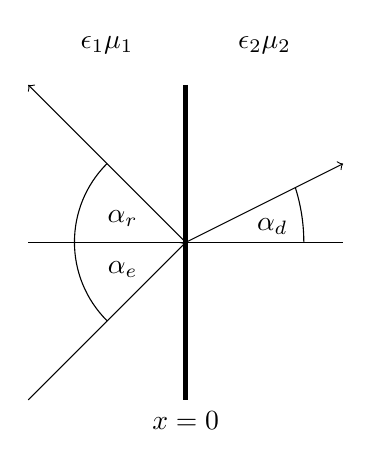
\begin{tikzpicture}
			\draw[ultra thick] (0,2)--(0,-2)node[below]{$x=0$};
			\draw (-2,0)--(2,0);
			\draw[->] (0,0)--(-2,2);
			\draw[->] (-2,-2)--(0,0);
			\draw[->] (0,0)--(2,1);
			\draw (-1,1) arc(135:225:1.41cm);
			\draw (1.5,0) arc(0:17.5:2.3cm);
			\draw (-0.8,0.3) node{$\alpha_r$};
			\draw (-0.8,-0.35) node{$\alpha_e$};
			\draw (1.1,0.2) node{$\alpha_d$};
			\draw (-1,2.5) node{$\epsilon_1\mu_1$};
			\draw (1,2.5) node{$\epsilon_2\mu_2$};
			\end{tikzpicture}
		}
	}
	\caption{Reflexion und Brechung}
\end{wrapfigure}
Um die Phänomene der Brechung und Reflexion zu untersuchen betrachten wir die folgenden Strahlen/Wellen:
\begin{align*}
\text{Einfallend:}\quad &\vec{E}^e e^{i(\vec{k}_e\vec{r}-\omega_e t)} &\qquad \omega_e =\frac{c}{n_1}k_e \\
\text{Reflektiert:}\quad&\vec{E}^r e^{i(\vec{k}_r\vec{r}-\omega_r t)} &\qquad \omega_r = \frac{c}{n_1}k_r \\
\text{Durchgehend:}\quad &\vec{E}^d e^{i(\vec{k}_d\vec{r}-\omega_d t)}&\qquad \omega_d=\frac{c}{n_2}k_d
\end{align*}
Natürlich muss $E_t$ bei $x=0$ stetig sein. 
\begin{equation*}
E_t^e e^{i(\vec{k}_e\vec{r}-\omega_e t)} + E_t^r e^{i(\vec{k}_r\vec{r}-\omega_r t)} = E_t^d e^{i(\vec{k}_d\vec{r}-\omega_d t)}
\end{equation*}
Wir sehen, so dass die $\omega_i$ im ganzen Raum identisch sein müssen. Genauso verhält es sich jeweils mit $k_{iy}$ und $k_{iz}$. Das gilt für beliebige Grenzflächenbedingungen! Aufgrund der Geometrie sehen wir nun
\begin{equation*}
k_{ey}=k_e\sin\alpha_e\ \stackrel{!}{=}\ k_{ry} = k_r\sin\alpha_r\ \stackrel{!}{=}\
k_{dy}=k_d\sin\alpha_d.
\end{equation*}
Mit $\omega_e=\omega_r=\omega_d$ und $\omega=\frac{c}{n}k$ folgt
\begin{align*}
k_e&=k_r &\frac{k_e}{n_1}&=\frac{k_d}{n_2}.
\end{align*}
So erhalten wir das \textbf{Reflexions- und Brechungsgesetz}
\begin{empheq}[box=\highlightbox]{align*}
\sin\alpha_e &=\sin\alpha_r &\frac{\sin\alpha_e}{\sin\alpha_d}&=\frac{n_2}{n_1}= \frac{c_1\vphantom{\big|}}{c_2\vphantom{\big|}}
\end{empheq}
Im folgenden schreiben wir $k_1$ für $k_e=k_r$, $k_2$ für $k_d$, sowie $\alpha$ für $\alpha_e=\alpha_r$ und $\beta$ für $\alpha_d$.\\

Werfen wir nun eine Blick auf das Verhalten der Amplituden an der Grenzfläche. Da $E_t$ und $H_t$ stetig sei müssen (keine Ströme!), also
\begin{align*}
E_t^e+E_t^r &= E_t^d\\
\frac{B_t^e}{\mu_1}+\frac{B_t^r}{\mu_1} &= \frac{B_t^d}{\mu_2}
\end{align*}
gelten muss und wir $\vec{B}=\frac{\vec{k}\times\vec{E}}{\omega}$ setzen können, ergibt sich
\begin{equation*}
\frac{(\vec{k}_e\times\vec{E}^e)_t}{\mu_1}+\frac{(\vec{k}_r\times\vec{E}^r)_t}{\mu_1} = \frac{(\vec{k}_d\times\vec{E}^d)_t}{\mu_2}.
\end{equation*}

\begin{enumerate}
\item \textbf{ senkrechter Einfall}\\

Der tritt mit $\alpha=0$ auf und so können wir, statt der Tangentialkomponenten auch einfach
\begin{equation*}
\vec{E}^e + \vec{E}^r = \vec{E}^d
\end{equation*}
schreiben. Es folgt außerdem
\begin{equation*}
\frac{k_1}{\mu_1}\left[\vec{e}_x\times\left(\vec{E}^e-\vec{E}^r\right)\right]_t = \frac{k_2}{\mu_2}\left[\vec{e}_x\times\vec{E}^d\right]_t,
\end{equation*}
was sogar auch ohne das Ziehen der Tangentialkomponente ( $]_t$ ) erfüllt wäre, da die Wellen transversal sind. 
\begin{equation*}
\frac{k_1}{\mu_1}\left(\vec{E}^e-\vec{E}^r\right) = \frac{k_2}{\mu_2}\vec{E}^d
\end{equation*}
Wir nehmen nun $\vec{E}^r=a^r\vec{E}^e$ und $\vec{E}^d=a^d\vec{E}^e$ an. Es wird sich später herausstellen, dass dadurch kein Widerspruch in der Gleichung entsteht. Setzen wir sie ein, erhalten wir
\begin{align*}
1+a^r&=a^d\\
1-a^r&=\frac{\mu_1k_2}{\mu_2k_1}a^d=:\nu a^d
\end{align*}
mit
\begin{equation*}
\nu:=\frac{k_2\mu_1}{k_1\mu_2}=\frac{n_2\mu_1}{k_1\mu_2}=\sqrt{\frac{\mu_1\epsilon1}{\mu_2\epsilon_2}}.
\end{equation*}
Wir erhalten damit die \textbf{\textsc{Fresnel}'schen Formeln für senkrechten Einfall}
\begin{empheq}[box=\highlightbox]{align*}
a^d&=\frac{2\vphantom{\big|}}{1+\nu\vphantom{\big|}} & a^r &=\frac{1-\nu}{1+\nu}.
\end{empheq}
Achtung: Bei Reflexion am dichten Medium kann in $a^r$ ein Phasensprung entstehen.\\
\newpage
\item \textbf{ Schräger Einfall}\\

Die eben gesehenen \textsc{Fresnel}-Gleichungen lassen sich für beliebige Winkel verallgemeinern (hier Rechnung). Man unterscheidet dabei, ob $\vec{E}$ senkrecht oder parallel zur Einfallsebene, die von einfallendem, reflektierten und durchgelassenem Strahl aufgespannt wird, steht.
\begin{empheq}[box=\highlightbox]{align*}
a_\perp^d&=\frac{2\vphantom{\big|}}{1+\nu\xi} & a_\perp^r&=\frac{1-\nu\xi}{1+\nu\xi}\\
a_\parallel^d&=\frac{2}{\xi+\nu\vphantom{\big|}} &a_\parallel^r &=-\frac{\xi-\nu}{\xi+\nu}
\end{empheq}
Dabei ist
\begin{equation*}
\xi=\frac{\cos\beta}{\cos\alpha}.
\end{equation*}

\item \textbf{ Energiebilanz für senkrechten Einfall}\\

Man erwartet natürlich
\begin{equation*}
S^e=S^d+S^r.
\end{equation*}
Es gilt auf jeden Fall
\begin{equation*}
|\vec{S}_P|=\frac{|\vec{E}\times\vec{B}|}{´\mu}=\frac{kE^2}{\omega\mu}=\frac{n}{c}\frac{E^2}{\mu}.
\end{equation*}
Daraus gewinnt man
\begin{align*}
cS_P^e &=\frac{n_1}{\mu_1}\left(E^e\right)^2 \\
cS_P^r &= \frac{n_1}{\mu_1}\left(a^rE^e\right)^2 = \left(a^t\right)^2cS_P^e\\
cS_P^d &=\frac{n_2}{\mu_2}\left(a^dE^e\right)^2 = \frac{n_1}{\mu_1}\nu\left(a^dE^e\right)^2 = \nu\left(a^d\right)^2cS_P^e=\left(1-\left(a^r\right)^2\right)cS_p^e.
\end{align*}
Zusammengefasst ist das
\begin{equation*}
S_P^d=S_P^e-S_P^r=TS_P^e
\end{equation*}
Man führt dann zum sogenannten \textbf{Transmissionskoeffizienten} $T$ noch den \textbf{Reflexionskoeffizienten} $R=\left(a^r\right)^2$ ein. Es gilt offensichtlich
\begin{equation*}
R+T=1.
\end{equation*}
\end{enumerate}


\section{Totalflexion}

Beim Übergang vom optisch dichteren ins optisch dünnere Medium ($n_2<n_1$) kann es zum Phänomen der Totalflexion kommen, bei dem ein eintreffender Strahl so stark vom Lot weggebrochen wird, dass er in der Grenzfläche liegt. Diesen Grenzwinkel liefert das Brechungsgesetz:
\begin{empheq}[box=\highlightbox]{equation*}
\sin\alpha_G = \frac{n_2\vphantom{\big|}}{n_1\vphantom{\big|}}
\end{empheq}
Für alle $\alpha > \alpha_G$ wird $\sin\beta>1$ und es gibt keine gebrochene Welle mehr. Die korrekte physikalische Interpretation ist
\begin{equation*}
\sin\beta=\frac{k_{2y}}{k_2}>1.
\end{equation*}
Mit $k^2=k_{2x}^2+k_{2y}^2$ folgt, dass $k_{2x}$ rein imaginär werden muss (wir schreiben $k_{2x}=i\kappa$). Das Feld im zweiten Medium hinter der Grenzfläche ist damit
\begin{equation*}
\vec{E}=\vec{E}^d e^{i(k_{2y}y-\omega t)}e^{-\kappa t}.
\end{equation*}
Die Welle parallel zur Oberfläche klingt also in $x$-Richtung exponentiell schnell ab. Es findet keine Dissipation statt, stattdessen wird die gesamte Energie reflektiert.\\
Das lässt sich auch anhand der \textsc{Fresnel}schen Formeln nachvollziehen. $\xi$ wird nämlich in dem Fall auch rein imaginär.
\begin{equation*}
\xi = \frac{\sqrt{1-\sin^2\beta}}{\cos\alpha}=:i\xi'
\end{equation*}
So werden die Formeln zu
\begin{align*}
a_\perp^r &=\frac{1-i\nu\zeta'}{1+i\nu\zeta'} &\Rightarrow& &|a_\perp^r|=1\\
a_\parallel^r &= -\frac{i\zeta'-\nu}{i\zeta'+\nu} &\Rightarrow& &|a_\parallel^r|=1
\end{align*}
Es wird also alles reflektiert, jedoch mit Phasenverschiebung. \\
Aber Vorsicht: Obwohl es in $x$-Richtung keine propagierende Welle gibt, können $a_\perp^d$ und $a_\parallel^d$ verschieden von Null sein. Ist das Medium $n_2$ sehr dünn, kann es durchaus zur Transmission kommen.